\documentclass[]{../resources/final_report}
\usepackage{graphicx}
\usepackage[hidelinks]{hyperref}


%%%%%%%%%%%%%%%%%%%%%%
%%% Input project details
\def\studentname{Roger Milroy}
\def\reportyear{2019}
\def\projecttitle{Autonomous Micro Air Vehicles: Enhanced Navigation in GPS denied environments.}
\def\supervisorname{Sara Bernadini}
\def\degree{BSc (Hons) in Computer Science (Artificial Intelligence)}
\def\fullOrHalfUnit{Full Unit} % indicate if you are doing the project as a Full Unit or Half Unit
\def\finalOrInterim{Project Plan} % indicate if this document is your Final Report or Interim Report

\begin{document}

\maketitle

%%%%%%%%%%%%%%%%%%%%%%
%%% Declaration

% \chapter*{Declaration}

% This report has been prepared on the basis of my own work. Where other published and unpublished source materials have been used, these have been acknowledged.

% \vskip3em

% Word Count: 

% \vskip3em

% Student Name: \studentname

% \vskip3em

% Date of Submission: 

% \vskip3em

% Signature:

% \newpage

%%%%%%%%%%%%%%%%%%%%%%
%%% Table of Contents
\tableofcontents\pdfbookmark[0]{Table of Contents}{toc}\newpage

%%%%%%%%%%%%%%%%%%%%%%
%%% Your Abstract here

\begin{abstract}

  I am proposing to use the newly developed technique of Graphical Recurrent Inference Networks
  in order to improve state estimation in GPS denied environments. I will compare performance to 
  the technique developed by Engel, Sturm and Cremers. .cite.

  One of the key challenges of operating with Micro Air Vehicles (MAVs) is payload 
  and power constraints .cite. , both of which also limit onboard computation. In the 
  approach my Engel, Sturm and Cremers they communicate with an offboard laptop
  in order to overcome this issue. This however obviously introduces other issues
  such as range and latency. I would like to see whether using GRIN and a different
  platform will enable me to implement a similar system onboard the drone.

  This project will allow me to work with diverse technologies, including state
  of the art Deep Learning techniques as well as different hardware. This will 
  present challenges in integration that will enable me to develop skills that will
  trasfer into robotics in general which is an area that I would like to become 
  more involved with.

\end{abstract}
\newpage


%%%%%%%%%%%%%%%%%%%%%%
%%% Background Reading

\chapter{Background Reading}
\addcontentsline{toc}{chapter}{Background Reading}
\section{Sources}
I read the below listed books, papers and websites while considering my project. I have included a brief explanation of why I read them and how they relate to the project proposed.

\begin{itemize}
  \item \textbf{A Concise Introduction to Models and Methods for Automated Planning, Geffner and Bonet} \cite{Geffner:2013:CIM:2534474} -  I read this book while considering my project. In the end I decided not to use planning in my project and to focus instead on technologies that would enable better performance of drones that do use planning.
  \item \textbf{Artificial Intelligence: A Modern Approach, Russell and Norvig} \cite{Russell:2009:AIM:1671238} - As one of the key books on the subject of AI, I will be using this book as a reference throughout the project.
  \item \textbf{Camera-Based Navigation of a Low-Cost Quadrocopter, Engel et al.} \cite{CameraBasedNav}  - This paper outlines the technique that I want to try and improve upon. One of the key tasks will be to port their implmentation onto the platform that we are using.
  \item \textbf{Accurate Figure Flying with a Quadrocopter Using Onboard Visual and Inertial Sensing, Engel et al.} \cite{FigureFlying} - This paper extends the ideas in the previous paper and uses them to complete accurate figure flying. I will attempt the same in order to properly evaluate the two approaches.
  \item \textbf{Recurrent Inference Machines for Solving Inverse Problems, Putzky and Welling.} \cite{DBLP:journals/corr/PutzkyW17}  - This paper outlines the techniques used in GRIN and as such is part of the motivation for implementing this technique in this domain. GRIN at it's core is a technique for improving upon model based mathematical models by adding learned error correction.
  \item \textbf{DJI OSDK website} \cite{dji:OSDK}- This is the reference page for the OSDK with which I will be controlling the drone programmatically. This is obviously extremely important to the success of the project.
  \item \textbf{hku\_100\_gazebo, GitHub caochao39} \cite{caochao39} - This repository contains code and explanation for creating a working simulation of a Matrice 100 in Gazebo. I will attempt to use this package to simulate effectively the Matrice in Gazebo.
  \item \textbf{Medium webpage for setup of Gazebo, Tahsincan Kose.} \cite{kose_2019} - This article extends the above repository enabling Hardware In The Loop testing of the Matrice 100 in Gazebo.
\end{itemize}



%%%%%%%%%%%%%%%%%%%%%%
%%% Project Spec

\chapter{Project Specification}
\addcontentsline{toc}{chapter}{Project Specification}

\section{Term 1}

The first term will consist mainly of proof of concept programs and reports that will develop my competence with, and understanding of, the necessary technologies that my project involves. This includes some background theory as well as coding. This will serve to both verify that the project is achievable in its current form, the second is to ease the programming load in the second term.

\subsection{Proof of Concept Programs}

\begin{itemize}
  \item \textbf{Simulate Matrice 100 in Gazebo} - It is important to have a standalone simulation of the model in Gazebo as this will allow testing without having the physical drone.
  \item \textbf{Get sensor data from the model in Gazebo} - I will need access to the sensor data for higher level tasks so this will be very important.
  \item \textbf{Connect Matrice 100 to Gazebo and the OSDK} - I will be targeting deployment onto the Matrice 100 and so I will need to test using it in Gazebo at some point.
  \item \textbf{Connect a Rasperry Pi to Matrice 100 via the OSDK} - I am planning to use a Rasperry Pi as the compute platform. This is because of its power, light weight and relatively low power draw. I will need to establish communication between the drone and the Pi in order to retrieve data for computation and issue commands for control.
  \item \textbf{Control the model programmatically via OSDK and ROS} - All the later tasks rely on being able to programmatically control the quadcopter. This will be implemented using ROS and the DJI OSDK.
  \item \textbf{Write and train an RIM} - RIMs are at the heart of GRIN which is the core component of this project so I need to learn how to program the structure. This will be on a demonstrator task.
\end{itemize}

\subsection{Reports}
\begin{itemize}
  \item \textbf{Kalman Filters for Sensor Fusion} - Both of the methods I will be contrasting use Kalman Filters and Extended Kalman Filters to integrate different sensor data. I will explore the theory behind this approach to sensor fusion.
  \item \textbf{Graph Convolutions} - GRIN uses convolutions over graphs in order to integrate neural networks with existing model based approaches. I will explore the theory underlying it and how it will apply to implementing GRIN.
  \item \textbf{Applications of Navigation in GPS Denied Environments} - I will explore the current and potential applications of these techniques. What are the challenges in expanding operations in these environments. What might the impact of expanded applications be. This report will have some relevance towards the Professional Issues section of the Final Report.
  \item \textbf{Recurrent Inference Machines} - GRINs use RIMs which is another recently developed technique. I will explore the theory and present the key concepts and techniques I will need.
\end{itemize}

\section{Term 2}

The focus of the second term will be implementing the project. This will involve translating the experience, skills and knowledge gained in the first term into a functioning product.

\subsection{Milestones}
\begin{itemize}
  \item \textbf{Port Camera-Based Navigation of a Low Cost Quadrocopter to DJI OSDK} - This is the system that I wish to evaluate against. In the interests of having a fair comparison I will port over the existing code base (which is open source) from the Parrot.AR to the Matrice and Rasperry Pi. I am implementing this first as it is an already implemented solution that will require less work. This will reduce the risks of total project failure.
  \item \textbf{Implement and train GRIN for the state estimation algorithm chosen} - This is the core of the project.
  \item \textbf{Quantify computational load and train reduced size model if needed} - As the plan is to deploy the implementation onboard the drone, it is very important that the computational and therefore power load be minimal. If the power load is too high I will attempt to train a minimized model to a similar accuracy.
  \item \textbf{Test and evaluate performance in Gazebo} - This will form the main evaluation of the work done and will show how successful my project is in relation to the aims.
  \item \textbf{Test and evaluate on Matrice 100} - This will be a real world evaluation which will demostrate how representative the simulation results are and how robust the project is to real world issues.
\end{itemize}

\subsection{Reports}
\begin{itemize}
  \item \textbf{Graphical Recurrent Inference Networks} - This is the technique I am planning to use. The core concept is integrating existing model approaches to inference with neural approaches to achieve improve results. I will explore the theory and present the key concepts and techniques I will need.
  \item \textbf{Alternative Navigation Techniques} - It is important when implmenting a system like this that you examine and evaluate alternatives. This report will enumerate and evaluate a variety of alternative approaches and their relative advantages.
  \item \textbf{Vision Based Navigation Techniques} - I will also explore alternative vision based approach to this task. I will summarise their advantages and disadvantages, where they are most appropriate and how they relate to the project I am implementing.
\end{itemize}

\newpage

\section{Timing and Gantt Chart}

\subsection{Motivation}
The strategy I have chosen in planning my milestones is intentionally conservative. I am planning for a slow start due to the number and complexity of new technologies and concepts. Once those have been successfully learnt the pace will increase substantially.
There is also considerable risk in hardware interfacing so I am completing that phase as early as possible.
\linebreak
\linebreak
I have also allowed some time at the end of each term as a buffer. This is primarily because I understand the limitations of my work and timing estimates. This buffer zone should increase the likelihood of overall project success.
\vspace{20pt}

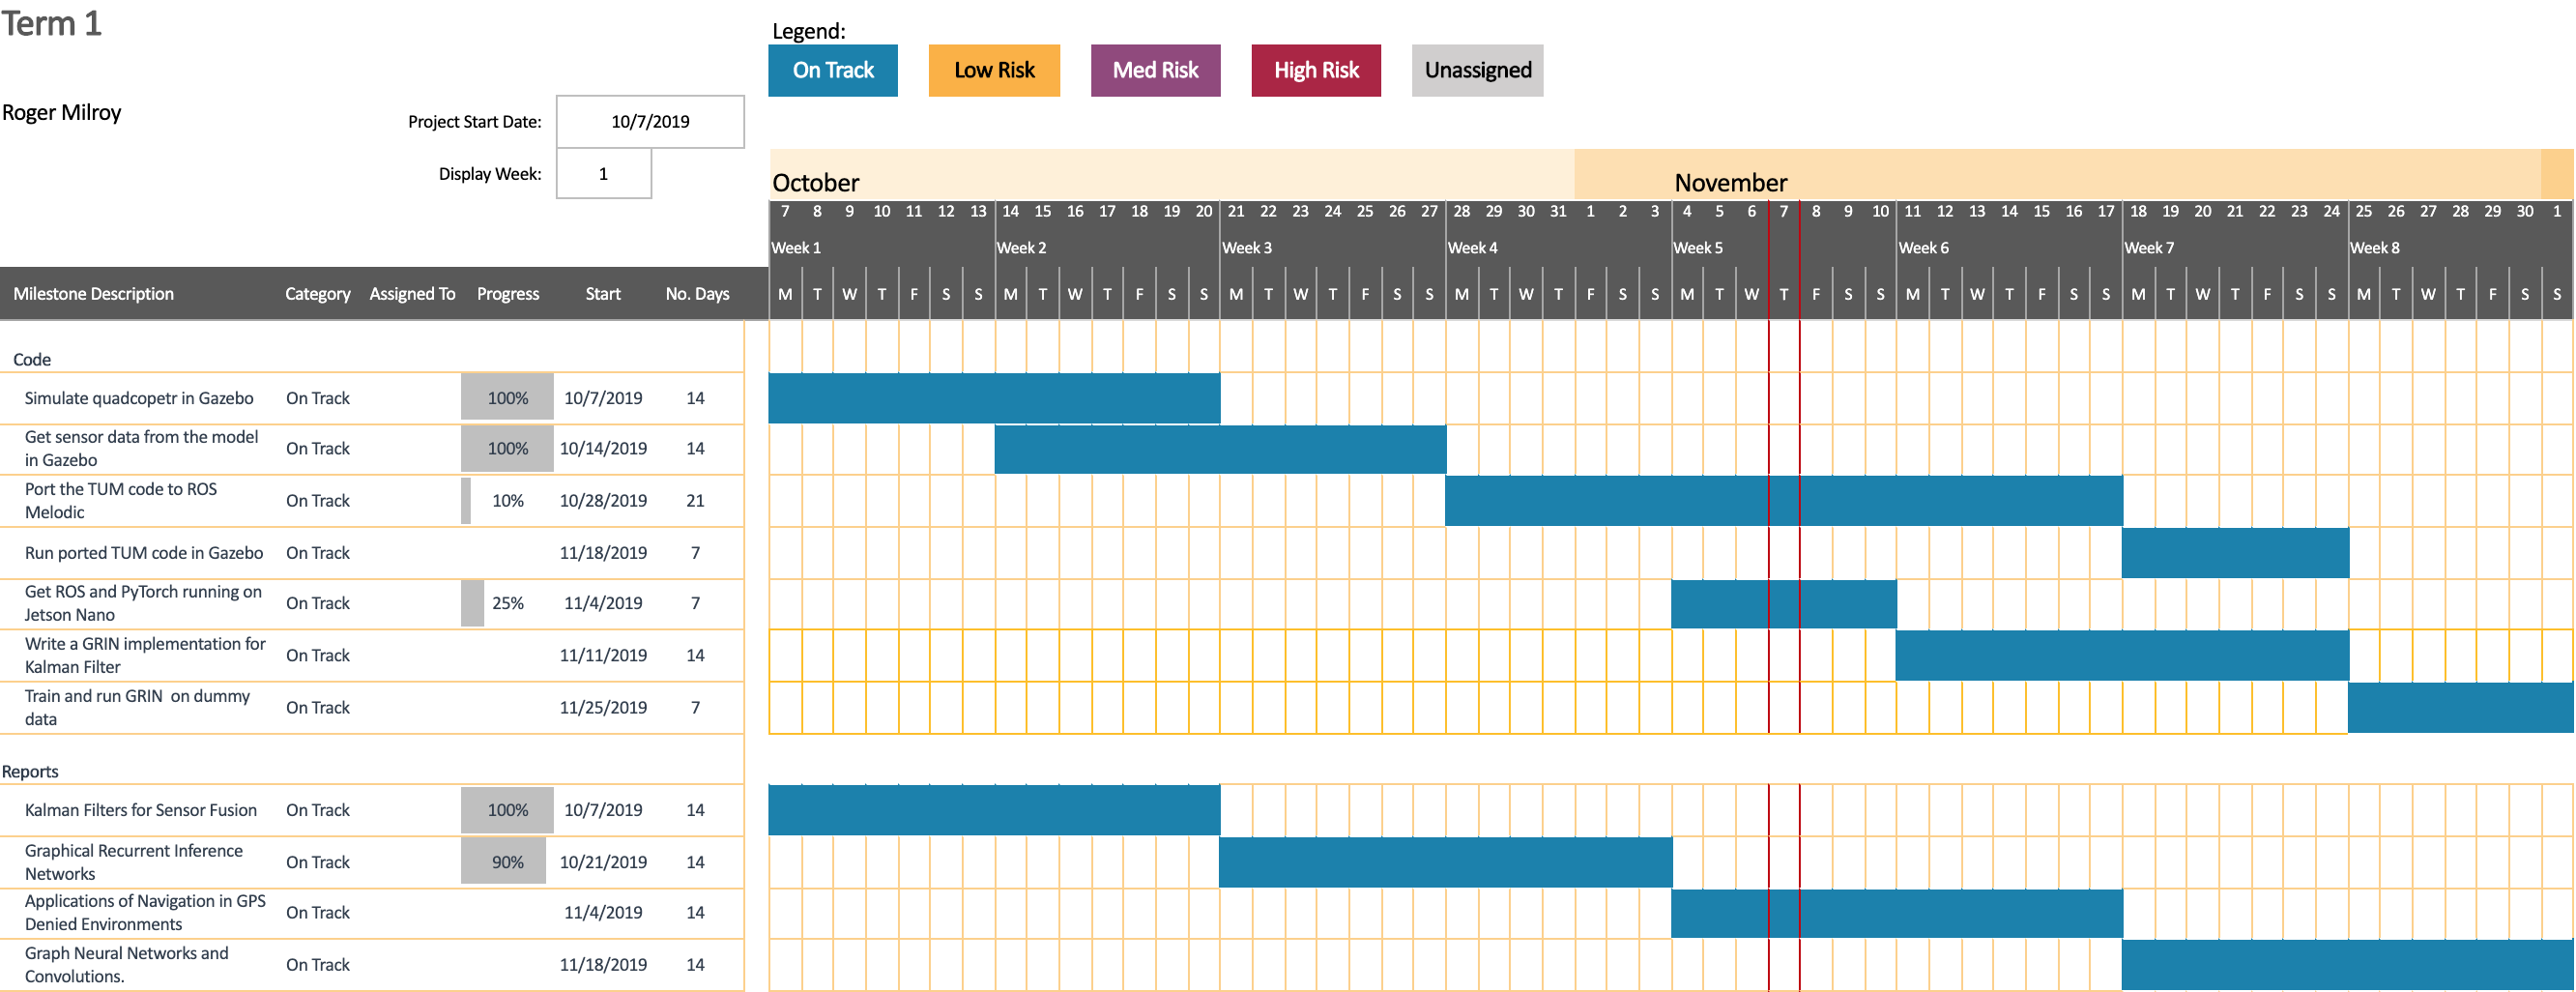
\includegraphics[width=\textwidth]{../resources/images/Term1GanttChart.png}

\vspace{20pt}

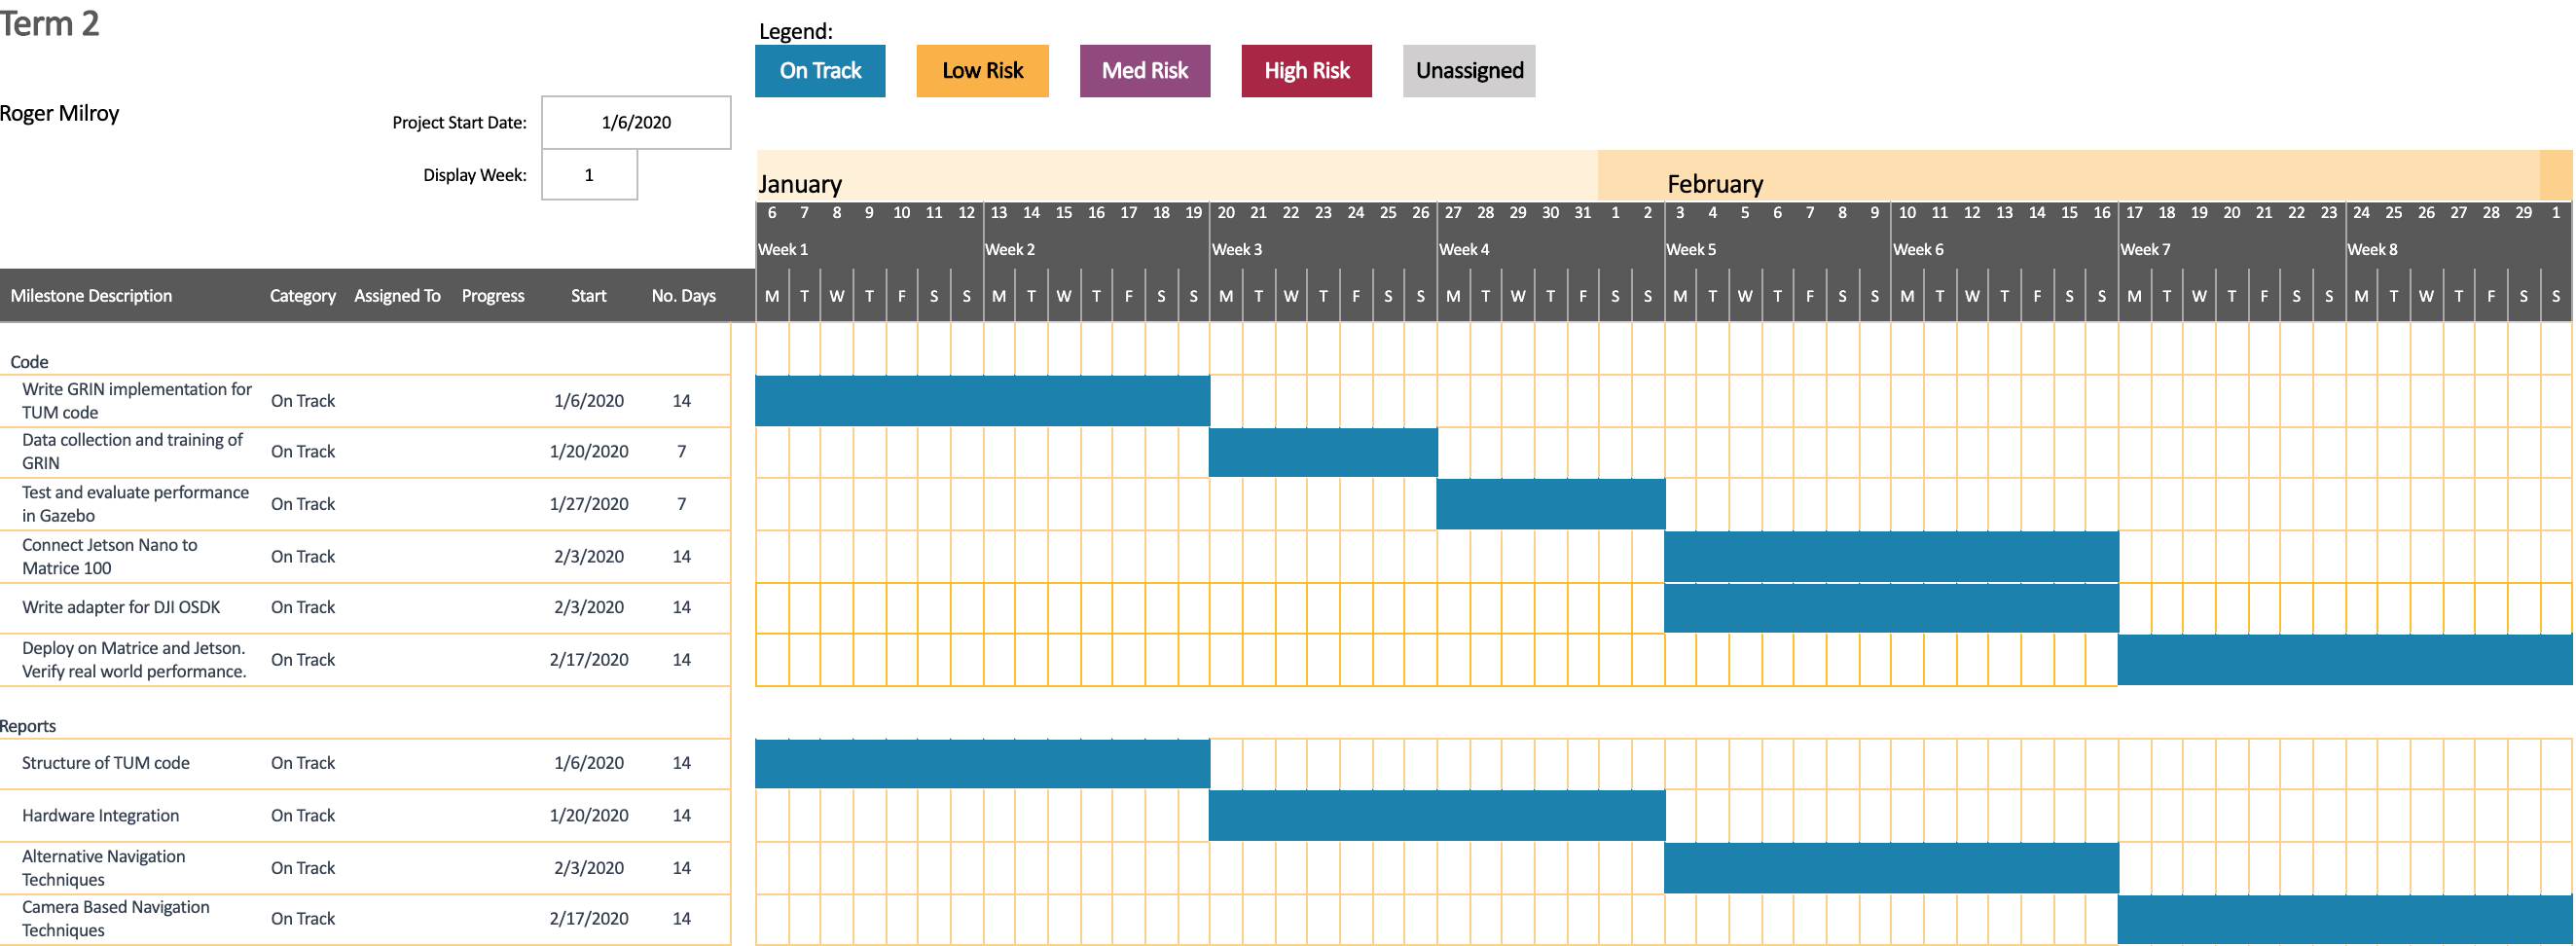
\includegraphics[width=\textwidth]{../resources/images/Term2GanttChart.png}


\chapter{Risks and Mitigation}

\section{Risks}
\subsection{Major Risks}

There are a few major risks to the success of the project.

\begin{itemize}
  \item \textbf{Access to information about GRIN.} - While information about RIMs is published and therefore publicly available, material about GRIN is currently unpublished. I have contacted the lead researcher to try to get access but this is by no means guaranteed. This presents the risk that I may have insufficient material to successfully implement the desired project.
  \item \textbf{Porting the existing code of Engel et al.} - As the project was targeted at a completely different platform there is no easy way to assess the difficulty of porting to our platform. This could mean that no comparison is possible.
  \item \textbf{Computational Load} - As the technique of GRIN is very new, there is no current analysis of the computational load. This may make it infeasible to deploy on a Raspberry Pi onboard the drone.
  \item \textbf{Resources for Training} - I am anticipating training the GRIN to take considerable computational resources. It is possible that I will have miscalculated the amount of resources I will need for this stage.
  \item \textbf{Overreach} - This is probably the key risk to this project. It is quite ambitious and presents the risk that the key element of the project will not be completed satisfactorily in time.
\end{itemize}


\subsection{Minor Risks}

\begin{itemize}
  \item \textbf{Access to the Drone} - There is only one drone between 4 students. This will mean time for development with the drone will be limited.
  \item \textbf{Hardware Issues} - As with any project involving hardware there exist a multitude of potential issues in the interface of hardware and software.
\end{itemize}

\pagebreak

\section{Mitigations}

As with all risks there are actions we can take to minimise the risks. At the same time it is a good idea to plan for the worst case scenario and have a good idea of how to recover and move forward.

\begin{itemize}
  \item \textbf{Access to information about GRIN.} - I will make the best use of my available resources to get in touch with the lead researcher in order to access the necessary information. If I am unable to get access I will pivot the project towards a direct comparison of a reinforcement learning based approach to compare with Engel et al.
  \item \textbf{Porting the existing code of Engel et al.} - One of my first tasks will be to assess the scale of the difference in code base, technologies and architecture. This should allow me to make an early determination if it is feasible or not. If it is not then I will shift from porting to reimplementing if that appears to be feasible. Again if not I will simply compare the results I am able to achieve directly to the results they present.
  \item \textbf{Computational Load} - It is entirely possible that GRIN will not be computationally feasible within the computational and time constraints. If this is the case, I will assess the possibility of transfer training a smaller network. I saw the possibility of this first in An On-device Deep Neural Network for Face Detection \cite{apple_machine_learning_journal_2017} and I would use the tips in Fitnets: Hints for thin deep nets \cite{Romero15fitnets:hints} if I get to this point. If that is still not possible then I will assess the possibility of using a remote computer, this is not however desireable.
  \item \textbf{Resources for Training} - I am planning  to use credits that I have available for AWS towards this. If this proves insufficient I may ask the department for assistance with access to GPU instances.
  \item \textbf{Overreach} - In order to minimise this risk I have already made some decisions relating to timing that I outlined above. In addition to this I have organised the project so that I am being as incremental as possible with lower risk elements coming first so that I should have deliverables to demonstrate even in the worst case. 
  \item \textbf{Access to the Drone} - This risk is entirely manageable. The first term will largely not require physical access to the drone and where possible I will be using simulations to reduce dependency further. In any case it shouldn't be too hard to organise access when needed.
  \item \textbf{Hardware Issues} - These are quite hard risks to remove in that they are mostly unknown and dealing with them will largely have to be reactive. That being said I will be verifying various levels of the different hardware in the first term in order to get ahead of any potential issues. I should have a good handle on the hardware by the end of the first term and therefore be better able to plan a hardware strategy for the second term.
\end{itemize}

%
%%%% ADD YOUR BIBLIOGRAPHY HERE
\newpage
\bibliographystyle{acm}
\bibliography{../resources/final_project}

\label{endpage}



\end{document}

\end{article}
